\section{解的性质}
\label{sec:heat-properties}

上面几节的解都有公式，公式只存在于少数几何形状上。一般区域、一般数据时能断定什么？下面研究四个量：总热量、最高最低温度、平方积分、光滑程度。每个量的变化规律都来自对方程本身的一次计算，不需要解的表达式，并且在估计中明确写出需要什么边界和源项条件。

\subsection{质量变化}
\label{sec:heat-mass}

棒里的总热量会怎样变？这是守恒律的积分形式，它的结论最直接。记$M(t)=\int_\Omega u(\bm{x},t)\,\mathrm{d}\bm{x}$。

\begin{theorem}[质量平衡]
\label{thm:heat-mass-balance}
设$\Omega$是有界开集，边界分段$C^1$，$u$在$\overline\Omega\times(0,T]$上有连续的$\partial_tu$和二阶空间偏导，满足$\partial_tu=\Delta u+f$，$f$连续。则对$0<t\leq T$，
\begin{equation}
 M'(t)=\int_\Omega f\,\mathrm{d}\bm{x}+\int_{\partial\Omega}\partial_{\bm{n}}u\,\mathrm{d}S .
 \label{eq:heat-mass-balance}
\end{equation}
\end{theorem}

\begin{proof}
被积函数连续，可以在积分号下对$t$求导：$M'(t)=\int_\Omega(\Delta u+f)\,\mathrm{d}\bm{x}$。由散度定理，$\Delta u=\nabla\cdot\nabla u$的体积分等于$\partial_{\bm{n}}u$的边界积分。这就是式~\eqref{eq:heat-mass-balance}。
\end{proof}

右端两项是两个不同的来源：内部源项的贡献和穿过边界的净通量。于是可以分情形读。

无源且零Neumann条件时，右端为零，总质量守恒。无源且零Dirichlet条件时，边界项一般不为零。设$u\geq0$，边界上$u=0$是最小值，温度沿外法向下降，$\partial_{\bm{n}}u\leq0$，所以$M'\leq0$，这种吸收边界让质量流失。

全空间没有边界，但需要无穷远处的衰减代替它。最直接的条件是$u_0\in L^1(\mathbb{R}^{d})$，这时由Fubini定理和$\int G=1$，
\[
 \int_{\mathbb{R}^{d}}u(\bm{x},t)\,\mathrm{d}\bm{x}=\int_{\mathbb{R}^{d}}u_0(\bm{y})\int_{\mathbb{R}^{d}}G(\bm{x}-\bm{y},t)\,\mathrm{d}\bm{x}\,\mathrm{d}\bm{y}=\int_{\mathbb{R}^{d}}u_0(\bm{y})\,\mathrm{d}\bm{y} .
\]
这里不需要任何关于导数在无穷远的假设。如果想用式~\eqref{eq:heat-mass-balance}在大球上取极限，就要证明大球面上的通量趋于零，这正是“适当衰减”的含义。

回到三角形。由式~\eqref{eq:heat-sine-solution}逐项积分，Dirichlet情形的质量是
\[
 M(t)=\sum_{k\text{ 奇}}\frac{8\sin(k\pi/2)}{k^3\pi^3}\,\mathrm{e}^{-k^2\pi^2t} .
\]
$t=0$时求和得$1/4$，$t=0.02,0.05,0.1,0.2$时依次约为
\[
 0.2102,\quad 0.1574,\quad 0.0962,\quad 0.0358 .
\]
Neumann情形$M$恒为$1/4$。对称性使两端的流出相同，式~\eqref{eq:heat-mass-balance}给出$M'=-2\partial_xu(0,t)$，$t=0.1$时左端斜率约为$0.4745$，流出率约为$0.949$，图~\ref{fig:heat-mass-balance}(b)用$M$的差商核对了这个等式。

有源时两项相互竞争。图~\ref{fig:heat-mass-balance}(c)取$f=1$，$u_0=0$。Dirichlet情形下，随着温度升高，边界流出变大，最终内部注入速率$1$被两端流出抵消，每端的斜率大小是$1/2$，质量趋于稳态的积分$\int_0^1x(1-x)/2\,\mathrm{d}x=1/12$。Neumann情形没有出口，$M(t)=t$无限增长，没有稳态，这对应着椭圆Neumann问题的相容条件$\int f=0$不成立。

\begin{BookInlineFigure}
  \centering
  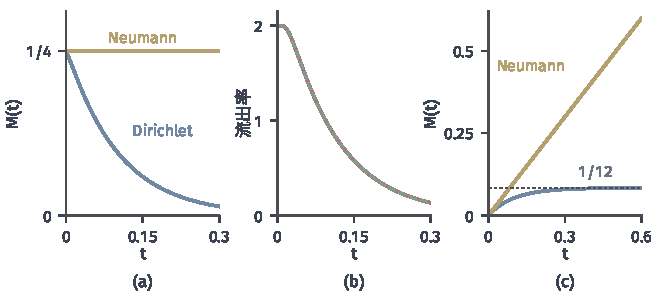
\includegraphics[width=112mm]{figures/06-differential-equations/02-partial-differential-equations/matplotlib/heat-mass-balance/figure.pdf}
  \caption{总热量的变化。(a)三角形初值、无源：Dirichlet（蓝）流失，Neumann（黄）不变。(b)Dirichlet情形的边界流出率$2\partial_xu(0,t)$（红）与$-M'(t)$的差商（绿色虚线），两者重合。(c)$f=1$、$u_0=0$：Dirichlet（蓝）趋于$1/12$，Neumann（黄）线性增长。}
  \label{fig:heat-mass-balance}
\end{BookInlineFigure}

\subsection{最大值原理}
\label{sec:heat-maximum}

没有热源时，棒内能不能出现比开始时和端点都热的点？物理上不能，热量只往低处流。数学上的结论需要指明温度的最大值可能出现在哪些地方，这就要看时空区域的边界中哪一部分真正影响解。

\paragraph{抛物边界}
记$\Omega_T=\Omega\times(0,T]$。称底面与侧面的并
\[
 \Gamma_T=(\overline\Omega\times\{0\})\cup(\partial\Omega\times[0,T])
\]
为\term{抛物边界}（parabolic boundary），它就是给定数据的那部分，图~\ref{fig:heat-parabolic-boundary}。顶面$t=T$不在其中，因为信息只从过去流向未来，那里的值由方程决定。

\begin{BookInlineFigure}
  \centering
  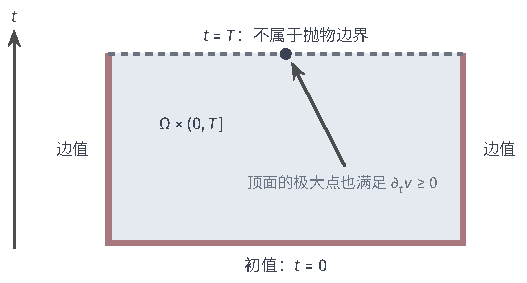
\includegraphics[width=90mm]{figures/06-differential-equations/02-partial-differential-equations/tikz/heat-parabolic-boundary/figure.pdf}
  \caption{时空矩形$\Omega\times(0,T]$的抛物边界（红色粗线）由底面和两条侧边组成，顶面（虚线）不属于它。顶面上若有极大点（黑点），那里的时间导数只能从过去一侧计算，符号仍然与方程矛盾，这正是定理的证明要点。}
  \label{fig:heat-parabolic-boundary}
\end{BookInlineFigure}

\begin{theorem}[弱最大值原理]
\label{thm:heat-weak-max}
设$\Omega$是有界开集，$u\in C(\overline\Omega\times[0,T])$，在$\Omega_T$上$\partial_tu$和二阶空间偏导连续，且$\partial_tu-\Delta u\leq0$。则
\begin{equation}
 \max_{\overline\Omega\times[0,T]}u=\max_{\Gamma_T}u .
 \label{eq:heat-weak-max}
\end{equation}
\end{theorem}

\begin{proof}
如果严格不等式$\partial_tv-\Delta v<0$成立，论证很短，所以先制造严格性。任取$\varepsilon>0$，令$v=u-\varepsilon t$，则
\[
 \partial_tv-\Delta v=\partial_tu-\Delta u-\varepsilon<0 .
\]
$v$在紧集上连续，在某点$(\bm{x}_0,t_0)$取得最大值。假设这一点不在$\Gamma_T$上，即$\bm{x}_0\in\Omega$，$0<t_0\leq T$。

固定$t_0$，$\bm{x}_0$是$v(\cdot,t_0)$的内部极大点，Hessian半负定，于是$\Delta v(\bm{x}_0,t_0)\leq0$。固定$\bm{x}_0$看时间：若$t_0<T$，一阶条件给出$\partial_tv=0$；若$t_0=T$，$v(\bm{x}_0,t)\leq v(\bm{x}_0,T)$对$t<T$成立，左导数给出$\partial_tv\geq0$。无论哪种情形，
\[
 \partial_tv-\Delta v\geq0,
\]
与严格不等式矛盾。所以$v$的最大值在$\Gamma_T$上取到。由$0\leq\varepsilon t\leq\varepsilon T$，
\[
 \max u\leq\max v+\varepsilon T=\max_{\Gamma_T}v+\varepsilon T\leq\max_{\Gamma_T}u+\varepsilon T .
\]
令$\varepsilon\to0$，得$\max u\leq\max_{\Gamma_T}u$。反方向的不等式成立是因为$\Gamma_T$是整个闭集的子集。
\end{proof}

条件$\partial_tu-\Delta u\leq0$的含义是内部不产生热量，可以吸热。对$-u$用定理，就得到$\partial_tu-\Delta u\geq0$时最小值在$\Gamma_T$上取到。图~\ref{fig:heat-max-envelope}中初值是$\sin(\pi x)+\sin(5\pi x)$，负的小凹陷很快被填平，最大值单调下降，最小值从$-0.198$上升到$0$，都不越出初值和边界值的范围。

\begin{BookInlineFigure}
  \centering
  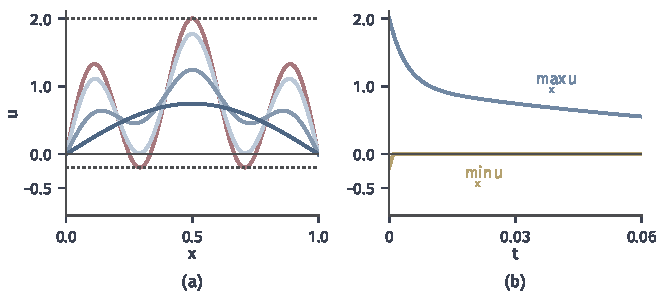
\includegraphics[width=112mm]{figures/06-differential-equations/02-partial-differential-equations/matplotlib/heat-max-envelope/figure.pdf}
  \caption{最大值原理的例子，$u_0=\sin(\pi x)+\sin(5\pi x)$（红），两端为零。(a)$t=0.001,0.005,0.03$的解（蓝色由浅到深），两条点线是初值的最大值$2$和最小值$-0.198$。(b)$\max_xu$（蓝）单调下降，$\min_xu$（黄）单调上升到$0$。}
  \label{fig:heat-max-envelope}
\end{BookInlineFigure}

这里要注意定理比较的是抛物边界上的值。零Neumann条件下侧面的值未知，定理不能直接说最大值在底面。一维时可以用偶延拓把隔热端点变成对称的内部点，再用全空间的结论，就知道隔热棒的最高温也不超过初值的最高温。一般区域上的同一结论需要边界点处法向导数的符号引理，篇幅较长，读者可查阅抛物方程的教材。

\paragraph{比较、唯一与连续依赖}
线性方程的两个解相减仍是解，把弱最大值原理用在差上，立刻得到几条结论。

\begin{theorem}[比较原理与唯一性]
\label{thm:heat-comparison}
设$\Omega$是有界开集，$u_1,u_2$满足定理~\ref{thm:heat-weak-max}的正则性，记$Lu=\partial_tu-\Delta u$。
\begin{enumerate}
 \item 若在$\Omega_T$上$Lu_1\leq Lu_2$，在$\Gamma_T$上$u_1\leq u_2$，则处处$u_1\leq u_2$。
 \item 若$Lu_i=f_i$，记$F=\sup_{\Omega_T}\lvert f_1-f_2\rvert$，则
 \begin{equation}
  \max\lvert u_1-u_2\rvert\leq\max_{\Gamma_T}\lvert u_1-u_2\rvert+TF .
  \label{eq:heat-max-stability}
 \end{equation}
 \item 特别地，Dirichlet初边值问题的经典解至多一个。
\end{enumerate}
\end{theorem}

\begin{proof}
(1)对$u_1-u_2$用定理~\ref{thm:heat-weak-max}。

(2)令$w=u_1-u_2-Ft$，则$\partial_tw-\Delta w=f_1-f_2-F\leq0$。由定理~\ref{thm:heat-weak-max}和$-Ft\leq0$，
\[
 \max(u_1-u_2)\leq\max w+FT\leq\max_{\Gamma_T}(u_1-u_2)+FT .
\]
交换$u_1$与$u_2$得到另一方向。

(3)在式~\eqref{eq:heat-max-stability}中令数据相同，右端为零。
\end{proof}

比较原理使我们能用简单的函数夹住解。例如例~\ref{ex:heat-source-steady}中$f=1$、$u_0=0$：与$w=t$比较，$\partial_tw-\partial_x^2w=1=f$，抛物边界上$u\leq w$，于是$u\leq t$；再与稳态$x(1-x)/2$比较，又有$u\leq x(1-x)/2$。前面算出$t=0.05$时中点值是$0.0463$，确实不超过$0.05$，也不超过$0.125$。

\paragraph{全空间与增长限制}
有界区域的证明用到了最大值存在，这在全空间不再自动成立，结论本身也可能失败。存在一族Tikhonov解，由
\[
 u(x,t)=\sum_{m\geq0}\frac{x^{2m}}{(2m)!}\,\phi^{(m)}(t),\qquad \phi(t)=\mathrm{e}^{-t^{-\alpha}}\ (\alpha>1,\ t>0),\quad \phi(0)=0
\]
给出，它在实轴上满足热方程，初值为零，却不恒为零。这个例子的收敛性验证较长，读者可查阅偏微分方程的教材。它的增长比$\mathrm{e}^{ax^2}$还快，这是无穷远处传进来的“幽灵热量”。下面的定理说明，只要禁止这样的增长，最大值原理就恢复了。

\begin{theorem}[全空间的最大值原理]
\label{thm:heat-whole-max}
设$u\in C(\mathbb{R}^{d}\times[0,T])$，在$\mathbb{R}^{d}\times(0,T]$上$\partial_tu$和二阶空间偏导连续，$\partial_tu-\Delta u\leq0$，并存在常数$A,a>0$，使
\begin{equation}
 u(\bm{x},t)\leq A\,\mathrm{e}^{a\lvert\bm{x}\rvert^2},\qquad \bm{x}\in\mathbb{R}^{d},\ 0\leq t\leq T .
 \label{eq:heat-growth}
\end{equation}
若$M_0=\sup u_0<\infty$，则$u\leq M_0$处处成立。特别地，若两个解的绝对值都满足式~\eqref{eq:heat-growth}这样的界，初值相同则解相同。
\end{theorem}

\begin{proof}
先设$4aT<1$，取$\varepsilon>0$使$4a(T+\varepsilon)<1$，并记$a+\gamma=1/(4(T+\varepsilon))$，$\gamma>0$。固定$\bm{y}\in\mathbb{R}^{d}$、$\mu>0$，引入一个向无穷增长、满足方程的比较函数。记$\rho=T+\varepsilon-t>0$，令
\[
 w(\bm{x},t)=\rho^{-d/2}\exp\Bigl(\frac{\lvert\bm{x}-\bm{y}\rvert^2}{4\rho}\Bigr) .
\]
直接求导，$\partial_tw$和$\Delta w$都等于$\bigl(\tfrac{d}{2\rho}+\tfrac{\lvert\bm{x}-\bm{y}\rvert^2}{4\rho^2}\bigr)w$，所以$\partial_tw=\Delta w$。令$v=u-\mu w$，则$\partial_tv-\Delta v\leq0$。

在球$B_r(\bm{y})$上用定理~\ref{thm:heat-weak-max}，只需看抛物边界。底面上$w>0$，所以$v\leq u_0\leq M_0$。侧面$\lvert\bm{x}-\bm{y}\rvert=r$上，用式~\eqref{eq:heat-growth}和$\rho\leq T+\varepsilon$，
\[
 v\leq A\,\mathrm{e}^{a(\lvert\bm{y}\rvert+r)^2}-\mu\,(T+\varepsilon)^{-d/2}\,\mathrm{e}^{(a+\gamma)r^2} .
\]
$r\to\infty$时第二项的指数系数$a+\gamma$大于第一项的$a$，右端趋于$-\infty$，于是$r$足够大时$v\leq M_0$。

由定理~\ref{thm:heat-weak-max}，$v\leq M_0$在球内成立。在球心取值，得$u(\bm{y},t)\leq M_0+\mu\,w(\bm{y},t)$。$w(\bm{y},t)=\rho^{-d/2}$有界，令$\mu\to0$，得$u(\bm{y},t)\leq M_0$。

一般的$T$，把$[0,T]$分成长度不超过$1/(8a)$的小段，逐段应用上面的结论，每一段的初值都不超过$M_0$。唯一性：两个解的差及其相反数都满足定理的条件，初值的上确界为零，差恒为零。
\end{proof}

增长条件的常数$a$可以任意大，$T$也可以任意大，不过$\mathrm{e}^{a\lvert\bm{x}\rvert^2}$这样的阶不能放宽，Tikhonov解正好越过这条线。这与定理~\ref{thm:heat-convolution-smooth}的积分条件相呼应：两者都以Gauss函数的增长为界。

\subsection{能量估计}
\label{sec:heat-energy}

最大值原理控制的是最坏的一点，并且依赖边界上的符号。另一种度量是平方积分，它在两种齐次边界下都表现得很好，而且自然地连接到弱解。记$E(t)=\tfrac12\lVert u(\cdot,t)\rVert_2^2$。

\begin{theorem}[能量估计]
\label{thm:heat-energy}
设$\Omega$是有界开集，边界分段$C^1$，$u\in C(\overline\Omega\times[0,T])$，在$\overline\Omega\times(0,T]$上$\partial_tu$和二阶空间偏导连续，满足$\partial_tu=\Delta u+f$（$f$连续）及零Dirichlet条件或零Neumann条件。则对$0<t\leq T$，
\begin{equation}
 \frac12\frac{\mathrm{d}}{\mathrm{d}t}\lVert u\rVert_2^2+\lVert\nabla u\rVert_2^2=\langle f,u\rangle .
 \label{eq:heat-energy-identity}
\end{equation}
无源时，对$0<t\leq T$还有
\begin{equation}
 \frac12\lVert u(\cdot,t)\rVert_2^2+\int_0^t\lVert\nabla u\rVert_2^2\,\mathrm{d}s=\frac12\lVert u_0\rVert_2^2 .
 \label{eq:heat-energy-integrated}
\end{equation}
一般地，零Neumann时取$\mu=0$，零Dirichlet时取$\mu=1/C_P^2$，其中$C_P$是Poincaré常数，则
\begin{equation}
 \lVert u(\cdot,t)\rVert_2\leq\mathrm{e}^{-\mu t}\lVert u_0\rVert_2+\int_0^t\mathrm{e}^{-\mu(t-s)}\lVert f(\cdot,s)\rVert_2\,\mathrm{d}s .
 \label{eq:heat-energy-bound}
\end{equation}
\end{theorem}

\begin{proof}
用$u$乘方程并在$\Omega$上积分。由Green公式，
\[
 \int_\Omega u\,\Delta u\,\mathrm{d}\bm{x}=-\lVert\nabla u\rVert_2^2+\int_{\partial\Omega}u\,\partial_{\bm{n}}u\,\mathrm{d}S .
\]
两种边界条件都使边界积分为零，一种因为$u=0$，另一种因为$\partial_{\bm{n}}u=0$。这就是式~\eqref{eq:heat-energy-identity}。

无源时把式~\eqref{eq:heat-energy-identity}在$[\varepsilon,t]$上积分。令$\varepsilon\to0^+$，$u$在闭集上连续，$E(\varepsilon)\to E(0)$；由单调收敛定理，梯度项收敛，这样得到式~\eqref{eq:heat-energy-integrated}。

为了得到式~\eqref{eq:heat-energy-bound}，想对$\lVert u\rVert_2$求导，但它在零点不可微，所以任取$\varepsilon>0$，令$y=(\lVert u\rVert_2^2+\varepsilon)^{1/2}$。由式~\eqref{eq:heat-energy-identity}和Cauchy--Schwarz不等式，以及$\lVert\nabla u\rVert_2^2\geq\mu\lVert u\rVert_2^2$（Neumann时$\mu=0$，这个不等式平凡；Dirichlet时是Poincaré不等式），
\[
 y\,y'\leq-\mu\lVert u\rVert_2^2+\lVert f\rVert_2\lVert u\rVert_2 .
\]
两边除以$y>0$，用$\lVert u\rVert_2\leq y$和$\lVert u\rVert_2^2/y\geq y-\sqrt\varepsilon$，
\[
 y'\leq-\mu y+\mu\sqrt\varepsilon+\lVert f\rVert_2 .
\]
乘积分因子$\mathrm{e}^{\mu t}$积分，令$\varepsilon\to0$，就得到式~\eqref{eq:heat-energy-bound}。
\end{proof}

式~\eqref{eq:heat-energy-integrated}有两层含义。第一，能量单调下降，下降的量正是梯度的平方积分，起伏越大，耗散越快。第二，即使初值只属于$L^2$，梯度在时间上的平方积分也不超过$\tfrac12\lVert u_0\rVert_2^2$，这是后面平滑效应的积分形式。

在$(0,1)$上零Dirichlet时最优的$C_P=1/\pi$，式~\eqref{eq:heat-energy-bound}无源时就是式~\eqref{eq:heat-series-decay}，能量方法不用模式得到了同样的衰减率。

\paragraph{用于比较两组数据}
方程线性，两个解的差满足同类问题，把式~\eqref{eq:heat-energy-bound}用在差上就是对数据的连续依赖：
\begin{equation}
 \lVert u_1(t)-u_2(t)\rVert_2\leq\mathrm{e}^{-\mu t}\lVert u_{1,0}-u_{2,0}\rVert_2+\int_0^t\mathrm{e}^{-\mu(t-s)}\lVert f_1-f_2\rVert_2\,\mathrm{d}s .
 \label{eq:heat-energy-stability}
\end{equation}
数据相同则差为零，所以这也给出唯一性，并且包括零Neumann问题，这是弱最大值原理没有直接给出的。

\begin{example}[两组初值的差]
\label{ex:heat-energy-difference}
在$(0,1)$上取零边值，$u_{1,0}$为三角形，第二组初值是
\[
 u_{2,0}=u_{1,0}+\tfrac{1}{10}(\sin\pi x+\sin3\pi x) .
\]
差的初值范数是$\tfrac{1}{10}\sqrt{1/2+1/2}=0.1$，而差本身是
\[
 u_2-u_1=\tfrac{1}{10}\bigl(\mathrm{e}^{-\pi^2t}\sin\pi x+\mathrm{e}^{-9\pi^2t}\sin3\pi x\bigr) .
\]
由正交性，其范数是$\tfrac{1}{10}(\tfrac12\mathrm{e}^{-2\pi^2t}+\tfrac12\mathrm{e}^{-18\pi^2t})^{1/2}$，不超过上界$0.1\,\mathrm{e}^{-\pi^2t}$。
\end{example}

\paragraph{能量衰减与质量守恒}
能量和质量是两个不同的量，隔热棒把这一点显示得最清楚：总质量不变，能量仍在减少。由Cauchy--Schwarz不等式，$M^2\leq\lvert\Omega\rvert\,\lVert u\rVert_2^2$，等号当且仅当$u$为常数。所以在质量固定时，均匀分布的能量最小，扩散正是把温度推向这个最小能量的状态。

三角形的初始能量是$\tfrac12\int_0^1u_0^2\,\mathrm{d}x=1/24$。在隔热棒中，最终温度是$1/4$，最终能量是$\tfrac12(1/4)^2=1/32$。两者相差的$1/96$由式~\eqref{eq:heat-energy-integrated}全部以梯度平方的时间积分耗散掉。接冰水时，能量和质量都趋于零，图~\ref{fig:heat-energy-mass}(a)。

\begin{BookInlineFigure}
  \centering
  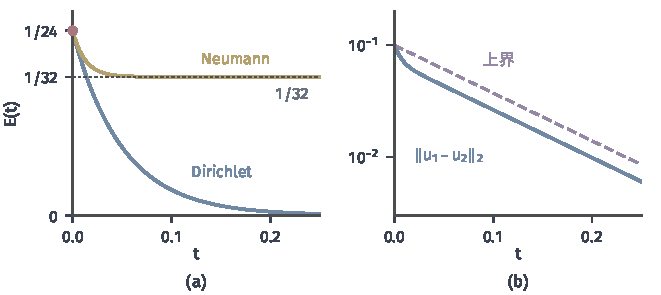
\includegraphics[width=112mm]{figures/06-differential-equations/02-partial-differential-equations/matplotlib/heat-energy-mass/figure.pdf}
  \caption{能量。(a)三角形初值（初始能量$1/24$，红点）的$E(t)$：Neumann（黄）下降到$1/32$后停止，Dirichlet（蓝）趋于$0$。(b)例~\ref{ex:heat-energy-difference}的差的$L^2$范数（蓝）与上界$0.1\,\mathrm{e}^{-\pi^2t}$（紫色虚线），纵轴为对数。}
  \label{fig:heat-energy-mass}
\end{BookInlineFigure}

上面的定理对经典解陈述。解也可以只在弱形式下成立：它在时间上平方可积地取值于$H^1_0(\Omega)$，对几乎每个$t$和每个$v\in H^1_0(\Omega)$有
\[
 \frac{\mathrm{d}}{\mathrm{d}t}\langle u,v\rangle+a(u,v)=\langle f,v\rangle ,
\]
其中$a(u,v)=\int_\Omega\nabla u\cdot\nabla v$，同样的能量等式仍然成立，取$v=u$的合法性需要取值于函数空间的时间导数理论，证明较长，读者可查阅抛物方程的教材。

表~\ref{tab:heat-three-measures}把三个度量放在一起。

\begin{BookInlineTable}
  \centering
  \caption{无源热方程的三种度量。}
  \label{tab:heat-three-measures}
  \begin{tabular}{llll}
    \toprule
    量 & 零Dirichlet & 零Neumann & 控制方式\\
    \midrule
    总质量 & 流失 & 守恒 & 边界通量\\
    最大值 & 不超过数据 & 不超过初值 & 符号结构\\
    能量 & 趋于$0$ & 趋于均匀态能量 & 梯度耗散\\
    \bottomrule
  \end{tabular}
\end{BookInlineTable}

\subsection{正时间平滑}
\label{sec:heat-smoothing}

定理~\ref{thm:heat-series}和定理~\ref{thm:heat-convolution-smooth}都说，$t>0$时解立即变成无穷光滑。这种\term{平滑效应}（smoothing effect）有多强？导数能大到什么程度？

\paragraph{全空间：把导数放到核上}
卷积的导数可以放在核上：$\partial^\alpha_{\bm{x}}u=(\partial^\alpha G)*u_0$。初值无需可导，所有的导数都由光滑的核承担，代价只是核的导数的大小。

\begin{theorem}[全空间的平滑估计]
\label{thm:heat-smoothing}
设$1\leq p\leq\infty$，$u_0\in L^p(\mathbb{R}^{d})$，$\alpha$是多重指标。则存在只依赖$\alpha$和$d$的常数$C_\alpha$，使对$t>0$，
\begin{equation}
 \lVert\partial^\alpha_{\bm{x}}u(\cdot,t)\rVert_p\leq C_\alpha\,t^{-\lvert\alpha\rvert/2}\,\lVert u_0\rVert_p .
 \label{eq:heat-smoothing}
\end{equation}
\end{theorem}

\begin{proof}
$L^p$函数满足式~\eqref{eq:heat-integrability}：由Hölder不等式，Gauss函数属于$L^{p'}$。于是定理~\ref{thm:heat-convolution-smooth}允许在积分号下求导。用定理~\ref{thm:heat-lp-recovery}证明中的Minkowski不等式，
\[
 \lVert\partial^\alpha u(\cdot,t)\rVert_p\leq\lVert\partial^\alpha G(\cdot,t)\rVert_1\,\lVert u_0\rVert_p .
\]
由尺度关系~\eqref{eq:heat-kernel-scaling}求导，
\[
 \partial^\alpha G(\bm{x},t)=t^{-(d+\lvert\alpha\rvert)/2}(\partial^\alpha G)(\bm{x}/\sqrt{t},1) .
\]
积分时代换$\bm{x}=\sqrt{t}\,\bm{z}$，因子$t^{d/2}$抵消，于是
\[
 \lVert\partial^\alpha G(\cdot,t)\rVert_1=t^{-\lvert\alpha\rvert/2}\lVert\partial^\alpha G(\cdot,1)\rVert_1 .
\]
把最后这个有限的$L^1$范数取作$C_\alpha$。
\end{proof}

一维$\alpha=1$时常数可以算出来。$G(\cdot,t)$是单峰函数，它的导数的$L^1$范数等于全变差，是峰值的两倍：
\[
 \lVert\partial_xG(\cdot,t)\rVert_1=2G(0,t)=\frac{1}{\sqrt{\pi t}} .
\]
于是
\[
 \lVert\partial_xu(\cdot,t)\rVert_\infty\leq\frac{\lVert u_0\rVert_\infty}{\sqrt{\pi t}} .
\]
这个常数不能再小：$u_0=\operatorname{sign}(x)$时$u=\operatorname{erf}(x/(2\sqrt{t}))$，在原点的斜率恰好是$1/\sqrt{\pi t}$，等号成立。

同样的办法还能把可积性换成有界性。卷积不超过核的上确界乘以$\lVert u_0\rVert_1$，于是
\[
 \lVert u(\cdot,t)\rVert_\infty\leq(4\pi t)^{-d/2}\lVert u_0\rVert_1 .
\]
这说明一点上的尖峰无法存留，只要总量有限，高度就被核的峰值控制。

\paragraph{区间：谱系数的压制}
有界区间上同样的结论由系数得到。对式~\eqref{eq:heat-sine-solution}，$\partial_x^mu$的系数比$u$多一个因子$(k\pi)^m$，而$\sqrt2\sin k\pi x$、$\sqrt2\cos k\pi x$都是标准正交系，所以
\[
 \lVert\partial_x^mu(\cdot,t)\rVert_2^2=\sum_k\lambda_k^m\,\mathrm{e}^{-2\lambda_kt}c_k^2\leq\Bigl(\sup_{\lambda>0}\lambda^m\mathrm{e}^{-2\lambda t}\Bigr)\sum_kc_k^2 .
\]
函数$\lambda^m\mathrm{e}^{-2\lambda t}$在$\lambda=m/(2t)$处取最大值，代入得到
\begin{equation}
 \lVert\partial_x^mu(\cdot,t)\rVert_2\leq\Bigl(\frac{m}{2\mathrm{e}\,t}\Bigr)^{m/2}\lVert u_0\rVert_2,\qquad t>0 .
 \label{eq:heat-spectral-smoothing}
\end{equation}
这和式~\eqref{eq:heat-smoothing}的$t^{-m/2}$一致。指数因子不管多小的$t$，都压得住任何多项式因子，这就是无穷光滑的来源；只是$t$越小，压制所需的频率越高，界就越大。

\paragraph{估计变差与初值的光滑性}
式~\eqref{eq:heat-smoothing}在$t\to0^+$时趋于无穷，这不说明解在变坏，而是说明界要为最粗糙的初值留有余地。初值的导数已经有界时，估计不必如此。

导数和卷积可交换：若$u_0$有界且一阶导数有界，则$\partial_xu=G*\partial_xu_0$，于是
\[
 \lVert\partial_xu(\cdot,t)\rVert_\infty\leq\lVert\partial_xu_0\rVert_\infty ,
\]
$t\to0^+$时没有奇性。解保持初值原有的光滑程度，只对超出这个程度的导数付出$t^{-1/2}$的代价。

图~\ref{fig:heat-smoothing-rates}用两个初值把这两件事分开。跳跃$\operatorname{sign}(x)$的一阶导数的界是$1/\sqrt{\pi t}$。折线$-\lvert x\rvert$的解满足$\partial_xu=-\operatorname{erf}(x/(2\sqrt{t}))$，一阶导数的界恒为$1$，二阶导数$\partial_x^2u=-2G(x,t)$的界是$1/\sqrt{\pi t}$：多出来的一阶导数才要付代价。跳跃的二阶导数代价是$t^{-1}$，正好多一个$t^{-1/2}$。

\begin{BookInlineFigure}
  \centering
  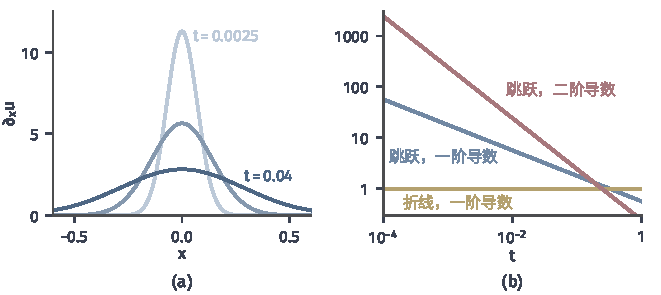
\includegraphics[width=112mm]{figures/06-differential-equations/02-partial-differential-equations/matplotlib/heat-smoothing-rates/figure.pdf}
  \caption{平滑的代价。(a)跳跃$\operatorname{sign}(x)$的解的斜率$2G(x,t)$，$t=0.0025,0.01,0.04$（蓝色由浅到深）。(b)精确的上确界，双对数坐标：跳跃的$\lVert\partial_xu\rVert_\infty=1/\sqrt{\pi t}$（蓝），跳跃的$\lVert\partial_x^2u\rVert_\infty\propto t^{-1}$（红），折线$-\lvert x\rvert$的$\lVert\partial_xu\rVert_\infty=1$（黄）。}
  \label{fig:heat-smoothing-rates}
\end{BookInlineFigure}
